% =====================================================================
%  CASTER -- Internship 2 Proposal
%  Ho Chi Minh City University of Technology (HCMUT), VNU-HCM
%  Faculty of Computer Science and Engineering
%
%  Build:  make         (latexmk -pdf main.tex)
%  Clean:  make clean
% =====================================================================
\documentclass[12pt,a4paper,oneside]{report}

% ---------- encoding / language ----------
\usepackage[T1]{fontenc}
\usepackage[utf8]{inputenc}
\usepackage[english]{babel}
\usepackage{lmodern}

% ---------- page geometry ----------
\usepackage[a4paper,left=3cm,right=2.5cm,top=3cm,bottom=3cm,headheight=28pt]{geometry}
\usepackage{setspace}
\onehalfspacing

% ---------- maths ----------
\usepackage{amsmath,amssymb,amsthm}
\usepackage{bm}

% ---------- tables / figures ----------
\usepackage{booktabs}
\usepackage{tabularx}
\usepackage{multirow}
\usepackage{array}
\usepackage{graphicx}
\usepackage{float}
\usepackage{caption}
\usepackage{subcaption}
\captionsetup{font=small,labelfont=bf}
\usepackage{longtable}

% ---------- misc ----------
\usepackage{enumitem}
\usepackage{xcolor}
\usepackage{fancyhdr}
\usepackage{titlesec}
\usepackage[hidelinks,breaklinks]{hyperref}
\usepackage{url}
\usepackage[numbers,sort&compress,super]{natbib}
\usepackage{pgfgantt}
\usepackage{textcomp}

\definecolor{bkblue}{HTML}{1F4E9C}
\hypersetup{colorlinks=true,linkcolor=black,citecolor=bkblue,urlcolor=bkblue}

% ---------- header / footer ----------
\pagestyle{fancy}
\fancyhf{}
\renewcommand{\headrulewidth}{0.8pt}
\fancyhead[R]{%
  \footnotesize\ttfamily
  \begin{tabular}{@{}r@{}}
    Ho Chi Minh City University of Technology\\
    Faculty of Computer Science and Engineering
  \end{tabular}%
  \IfFileExists{figures/bk-logo.pdf}{\raisebox{-2pt}{\includegraphics[height=22pt]{figures/bk-logo.pdf}}}{}%
}
\fancyfoot[C]{\thepage}
\fancypagestyle{plain}{\fancyhf{}\renewcommand{\headrulewidth}{0pt}\fancyfoot[C]{\thepage}}

% ---------- chapter headings ----------
\titleformat{\chapter}[display]
  {\normalfont\huge\bfseries}{\chaptertitlename\ \thechapter}{20pt}{\Huge}
\titlespacing*{\chapter}{0pt}{0pt}{30pt}

% ---------- shorthands used throughout ----------
\newcommand{\km}{\ensuremath{K/\hat{m}}}
\newcommand{\kmc}[1]{\ensuremath{K/\hat{m}^{\,#1}}}
\newcommand{\caster}{\textsc{Caster}}
\newcommand{\cegmem}{\textsc{CegMem}}
\newcommand{\frtp}{\textsc{Frtp}}
\newcommand{\code}[1]{\texttt{#1}}

\theoremstyle{definition}
\newtheorem{definition}{Definition}[chapter]

% ---------- cover-page details: edit metadata.tex, not this file ----------
% =====================================================================
%  EDIT THIS FILE -- cover-page details only. Nothing else reads them.
% =====================================================================

\newcommand{\StudentName}{Nguyen Thanh Trung Dat}   % <-- CHECK / EDIT
\newcommand{\StudentID}{0000000}                    % <-- EDIT
\newcommand{\InstructorName}{Dr. Le Xuan Bach, CSE-HCMUT}  % <-- CHECK / EDIT
\newcommand{\ReportMonth}{November 2026}


\begin{document}

% ======================= FRONT MATTER =======================
\pagenumbering{roman}
\begin{titlepage}
\thispagestyle{empty}
\centering

{\large\scshape
Vietnam National University Ho Chi Minh City\\[2pt]
Ho Chi Minh City University of Technology\\[2pt]
Faculty of Computer Science and Engineering\\
}

\vspace{2.2cm}

{\large\bfseries -- INTERNSHIP 2 REPORT --}

\vspace{1.4cm}

{\Huge\bfseries
Cost-Aware Validation Scheduling\\[6pt]
and Selected Hints for\\[6pt]
LLM-Based Program Repair\\
}

\vspace{1.0cm}

\IfFileExists{figures/bk-logo.pdf}{%
  \includegraphics[height=3.6cm]{figures/bk-logo.pdf}\par
}{\vspace{3.6cm}}

\vfill

{\large
\begin{tabular}{r@{\hskip 1em}l}
  Council:    & Computer Science and Engineering \\[3pt]
  Instructor: & \InstructorName \\[3pt]
  Student:    & \StudentName \\[3pt]
  Student ID: & \StudentID \\
\end{tabular}
}

\vspace{1.8cm}

{\large\scshape Ho Chi Minh City, \ReportMonth}

\end{titlepage}

\clearpage
\thispagestyle{empty}

\vspace*{6cm}

\noindent
\begin{minipage}[t]{0.52\textwidth}
  \rule{0.78\textwidth}{0.8pt}\\[2pt]
  \InstructorName\\
  Faculty of Computer Science and Engineering
\end{minipage}%
\hfill
\begin{minipage}[t]{0.40\textwidth}
  \raggedleft
  Date: \rule{3.2cm}{0.8pt}
\end{minipage}

\vfill


\setcounter{page}{3}
\chapter*{Acknowledgements}
\addcontentsline{toc}{chapter}{Acknowledgements}
\markboth{Acknowledgements}{Acknowledgements}

I would like to thank the lecturers of the Faculty of Computer Science and
Engineering, Ho Chi Minh City University of Technology (HCMUT), for the
foundational and specialised teaching that made this work possible.

I am especially grateful to my instructor, \InstructorName, for the guidance
that shaped the scope of this work. Two pieces of that guidance did most of the
work. The first was the insistence that a research question be stated together
with the outcome that would \emph{refute} it; applying that test removed several
items from an earlier list that turned out to be names for groups of experiments
rather than questions. The second was the instruction to measure the resource
the system actually spends rather than the one the literature happens to report,
which is why Chapter~\ref{ch:experiments} reports CPU seconds and test
executions side by side instead of either alone.

I also thank my colleagues for the discussions that sharpened the central
distinction this work is built on: that a repair loop learns two different
things on every iteration --- which test is worth running, and which repair idea
is already dead --- and that both are usually discarded.

This document reports work in progress. The implementation and its unit tests
are complete; the $100$-task pilot is running at the time of writing, and
Chapter~\ref{ch:results} marks every number that depends on it. Any remaining
errors are my own.

\chapter*{Abstract}
\addcontentsline{toc}{chapter}{Abstract}
\markboth{Abstract}{Abstract}

A large-language-model program-repair loop alternates between a proposer, which
draws a candidate patch, and an oracle, which refutes it by finding a test case
on which the patch is wrong. The proposer is the half that gets the attention
and the oracle is the half that costs. On the corpus studied here the oracle's
own reference program takes a median of 0.076\,s of CPU per test
case but a 99th percentile of 4.48\,s --- a spread of
$58.7\times$ inside the same pool --- and a loop that walks that pool in the
order the benchmark ships spends 2.18\,s of CPU per round, on every
round, for twenty rounds.

Existing memories for repair loops do not touch that cost. They are keyed by a
failure \emph{class}: fault-recorded testing prioritisation ranks a case by how
many patches it has already falsified, and the predecessor of this work,
\cegmem, stored each refuted patch under a type formed from its edit location
and the property it violated. A class-keyed memory can say which patches not to
try again --- \cegmem\ cut oracle calls per episode from $11.11$ to $1.57$,
a factor of $7.07$ --- but it cannot say which test to run first, and it cannot
say which test is cheap.

This proposal develops \caster, a repair loop whose memory is keyed by
\textbf{test case} rather than by failure class. Each case carries an online
Beta-posterior kill rate $K$ and an online mean CPU cost $\hat{m}$, and probes
are scheduled by the index \km: refute early, and refute cheaply. Keying on the
case is also what makes the second half possible, because a case is an
\emph{observation} and only an observation can be phrased to the proposer as a
positive requirement rather than a prohibition.

\paragraph{What this document reports as evidence.} The preliminary validation
is a pilot on the frozen data of the \cegmem\ study: $68$ ConDefects tasks,
$2{,}523$ test cases and $4{,}670$ stored patches for which a complete
patch~$\times$~case verdict matrix, a measured per-case reference CPU cost, and
a per-case coverage trace all exist. Two experiments run on it. A replay
simulation reproduces an arbitrary probe order exactly from the verdict matrix;
a second study re-executes the loop for real over $6{,}800$ rounds per policy
and measures CPU with \code{getrusage}. The measured result is that \km\ costs
\textbf{76.2\,\%} less oracle CPU than the shipped pool order
(95\,\% CI $[-84.9, -61.2]$, $p = 1.7\times10^{-11}$, cheaper on $63$ of $68$
tasks) and \textbf{15.7\,\%} less than the published
fault-recorded baseline (95\,\% CI $[-28.9, -5.1]$, $p = 0.011$, $42$ of $68$)
--- while paying 23.3\,\% \emph{more} probes than that baseline.
Executions and CPU therefore disagree in sign on this corpus, which matters
because the test-prioritisation literature deliberately reports executions.

\paragraph{What it does not report.} The \caster\ implementation itself has
been built and unit-tested but its experimental grid has not been run. The
twenty-two arms, the steered prompt contract that the test-case key is supposed
to enable, the duplicate-rate and token-cost measurements, and the full
fault corpus are Phase~2 work and are stated as such throughout. No number in
Chapter~\ref{ch:evaluation} is a result; every number there is a target.


\tableofcontents
\listoffigures
\listoftables

% ======================= MAIN MATTER ========================
\clearpage
\pagenumbering{arabic}
\setcounter{page}{1}

\chapter{Introduction}
\label{ch:intro}

\section{Problem Statement}
\label{sec:problem}

Automated program repair (APR) has converged on a loop with two halves. A
\emph{proposer} produces a candidate patch, and an \emph{oracle} decides
whether that candidate is wrong by running it against a pool of test cases and
looking for one on which it misbehaves~\citep{legoues2019apr}. In the
generate-and-validate tradition the proposer was a mutation
operator~\citep{legoues2012genprog}; today it is usually a large language
model~\citep{xia2024chatrepair}. The oracle has not changed: it is still a
sequence of program executions, and it is still the half that burns the
machine.

How much it burns is easy to under-estimate, because the usual unit of account
hides it. The test-prioritisation literature reports \emph{test executions}
rather than time, and does so deliberately: the largest recent study of patch
validation states that it presents results in executions because ``the number
of test executions is more stable and more suitable for future work to
reproduce''~\citep{lou2024aprregression}. That choice is sound when executions
are interchangeable. On the corpus studied in this proposal they are not. The
oracle's own reference program takes a median of 0.076\,s of CPU on
one test case and 4.48\,s at the 99th percentile --- a $58.7\times$
spread --- and the variation is not between easy and hard \emph{tasks} but
inside a single task's pool, where the median coefficient of variation of
per-case cost is $0.571$. Counting executions on such a pool is counting apples
and buses.

The consequence shows up directly in the loop. A repair loop that walks the
pool in the order the benchmark happens to ship --- which is what any
implementation gets for free, and therefore what most implementations do ---
spends 2.18\,s of oracle CPU per round and keeps spending it: the
cost per round is flat from round~1 to round~20, because nothing in the loop
learns anything about the pool. Over the $6{,}800$ rounds measured in
Section~\ref{sec:pilot} that order costs 14843\,s of CPU where a
scheduled order costs 3532\,s.

Two kinds of memory have been proposed to make the loop cheaper, and neither
addresses this. \emph{Fault-recorded testing prioritisation} (\frtp)
ranks a test case by the number of patches it has already
falsified~\citep{qi2013frtp}; the same quantity, under the name ``patch killing
count'', drives later variants~\citep{venugopal2020mpp}. \cegmem, the study
that precedes this one, went further and stored every refuted patch under a
\emph{failure type} formed from the patch's edit location and the property it
violated, so that a fresh candidate matching a stored type could be rejected
before the oracle was paid at all. That worked: it cut oracle calls per
episode from $11.11$ to $1.57$, a factor of $7.07$
(Section~\ref{sec:cegmem-premise}).

But both memories are keyed by a \emph{class}, and a class-keyed memory answers
only one of the two questions a repair loop asks. It can answer \emph{which
patches are not worth testing}. It cannot answer \emph{which test to run
first}, and it certainly cannot answer \emph{which test is cheap} --- \frtp's
whole family records that a case killed, never what the kill cost, and never
the evidence of a case failing to kill, which is the information that
distinguishes a case that spared ten patches from one that was never run. In
\cegmem\ the residual was plainly visible: the memory removed most oracle
\emph{calls}, yet the loop still performed $39.5$ sandbox executions per
episode and still spent 14.1\,s per episode inside the guard,
because every surviving call still walked the pool in alphabetical order.

This proposal targets that residual. The idea is to key the memory by
\textbf{test case} instead of by failure class, to learn two online quantities
per case --- a kill rate and a cost --- and to schedule probes by their ratio.
Keying on the case has a second consequence that motivates the rest of the
design: a test case is an \emph{observation}, and only an observation can be
handed back to the proposer as a positive requirement (``produce exactly this
output on this input'') rather than as a prohibition (``do not do that
again''). The scheduler and the prompt contract are therefore one system, and
they ship together.

\section{Research Objectives and Questions}
\label{sec:rq}

This research aims to design, implement and evaluate a repair loop whose
memory of refuted attempts is indexed by test case, and to establish how much
of the oracle's cost that indexing removes. Four objectives structure the
work; each is paired with the question it answers and, following the discipline
adopted throughout this project, with the outcome that would \emph{refute} it.
A question with no refuting outcome is a name for a group of experiments, not a
question.

\begin{enumerate}[leftmargin=*,itemsep=6pt]

\item \textbf{Cost-aware probe scheduling.} Schedule the oracle's probes by an
online per-case kill rate divided by an online per-case cost, rather than by
pool order or by a kill count.
\emph{Research question (RQ1).} Does scheduling by \km\ reduce the CPU spent
refuting a patch, measured against the incumbent pool order, against an
uninformed random control, and against the published prioritisers \frtp\ and
additional-greedy coverage?
\emph{Refuted when} \km\ is not cheaper than pool order beyond the cluster
bootstrap's interval; or when it is cheaper than pool order but not cheaper
than \frtp\ and coverage, in which case the contribution is early stopping,
which is not ours.
\emph{Status.} Answered in the affirmative by the pilot of
Section~\ref{sec:pilot}; to be re-established on the full corpus in Phase~2.

\item \textbf{Attribution of the effect.} Decompose the index into the three
things it adds to the incumbent --- having a memory at all, turning a count
into a rate, and dividing that rate by cost.
\emph{Research question (RQ2).} Which of the three terms produces the effect?
\emph{Refuted when} no single step clears the bootstrap interval, so the gain
is ``having any memory'' and the score is ornament; or when the cost division
alone carries it, in which case the kill rate is ornament.
\emph{Status.} Partially answered by the pilot's exponent sweep
(Section~\ref{sec:pilot-sweep}), which separates the kill term from the cost
term; the full stepwise ladder is Phase~2.

\item \textbf{Renormalising the patch family.} Return the scheduled
counterexample to the proposer as a positive requirement keyed to a test case.
\emph{Research question (RQ3).} Does doing so move the proposal distribution
off the mode it has already drawn --- fewer duplicate patches, more repairs at
the same budget --- where a conversation transcript and a prohibition do not?
\emph{Refuted when} the duplicate rate does not fall against independent
repeated sampling; or when it falls and the repair rate does not rise, in which
case the distribution moved somewhere no better.
\emph{Status.} Not addressed by the pilot. The baseline is set by published
measurement: independent repeated prompting has already been reported to repair
$23$ bugs against conversational repair's $18$ at an equal budget of $24$ model
calls, with $65\,\%$ of the conversational system's patches
duplicates~\citep{chen2025conversational}. Any steering arm must beat repeated
sampling, not the pool order.

\item \textbf{The disclosure dose.} Showing a counterexample tells the model
what to satisfy.
\emph{Research question (RQ4).} At what level of disclosure does the proposer
begin satisfying \emph{the shown probes} rather than repairing the fault?
\emph{Refuted when} the share of patches refuted only outside the disclosed set
is flat across the number of facts shown and across disclosure level, in which
case there is no dose and the axis does not exist.
\emph{Status.} Phase~2.

\end{enumerate}

\paragraph{Contribution positioning.} None of the individual ingredients is
new. Cost-cognizant prioritisation dates to \citet{elbaum2001cost}; the
additional-greedy family to \citet{rothermel2001prioritizing}; prioritisation
inside a repair loop to \citet{qi2013frtp}; and Beta-posterior estimates with
$\varepsilon$-greedy exploration are standard. The claim made here is at the
level of the \emph{key and the unit}. First, the memory is indexed by test
case, which is what lets one record serve both the scheduler and the prompt;
every memory in the surveyed repair literature is indexed by a class. Second,
the ranked quantity is a rate divided by a measured cost, where the published
repair-loop prioritiser ranks on a count and discards both the non-kills and
the cost. Third --- and this is the finding the pilot contributes rather than
the design --- on a pool with $58.7\times$ internal cost spread the two units
of account disagree in sign, so the deployment-facing claim cannot be read off
an execution count at all.

\section{Scope}
\label{sec:scope}

The study is bounded to the dimensions in Table~\ref{tab:scope}.

\begin{table}[H]
\centering
\caption{Project scope.}
\label{tab:scope}
\small
\begin{tabularx}{\textwidth}{@{}lX@{}}
\toprule
\textbf{Dimension} & \textbf{Specification}\\
\midrule
Task domain & Single-fault repair of competitive-programming submissions; one
faulty program, one contest test pool, stdout-compared verdicts.\\
Benchmark & ConDefects~\citep{wu2024condefects}, Python subset. Chosen because
every test input ships with the output the judge accepted, so a refutation is a
concrete input/output pair rather than a pass/fail bit.\\
Proposer & One OpenAI-compatible chat model per grid; \code{gpt-4o-mini} for
the data the pilot reuses. The proposer is not a variable of the study.\\
Oracle & One program, one input, hard timeout, CPU measured with
\code{getrusage(RUSAGE\_CHILDREN)}; probing stops at the first refutation.\\
Cost unit & CPU seconds as primary, test executions reported alongside.
Wall-clock time is never used as a cost, because it is contaminated by sibling
processes.\\
Core method & Per-case Beta-posterior kill rate $K$ over an online per-case
mean cost $\hat{m}$, ranked by \km, with $\varepsilon$-greedy exploration.\\
Evidence in this document & A replay and re-execution pilot on the frozen
\cegmem\ data: $68$ tasks, $2{,}523$ cases, $4{,}670$ patches,
$6{,}800$ measured rounds per policy.\\
Out of scope here & The \caster\ grid itself (22 arms), the steered prompt
contract, duplicate-rate and token measurements, multi-fault and multi-language
repair, and any claim about repair \emph{quality} beyond the soundness
invariant of Section~\ref{sec:soundness}.\\
\bottomrule
\end{tabularx}
\end{table}

\paragraph{Scope of completed work at the proposal stage.} The \caster\
implementation exists: ten command-line verbs, the module boundaries of
Section~\ref{sec:overview}, and $263$ unit tests that run without a network, a
model or the benchmark. What has \emph{not} happened is the experiment. No arm
of the grid has been run to completion on the full corpus, no steered arm has
been run at all, and therefore nothing in this document derived from the
\caster\ repository is reported as a result. The evidence is the pilot, and the
pilot runs on the previous project's data by design --- see
Section~\ref{sec:why-pilot-here} for why that is the stronger choice and not
merely the available one.

\section{Report Structure}

Chapter~\ref{ch:related} surveys validation-cost work along four families ---
generate-and-validate repair and its validation bill, regression test
prioritisation, repair-specific prioritisation, and the token economics of
LLM repair loops --- consolidates them into one comparison table, and states
the gaps. Chapter~\ref{ch:background} gives the theory: the two costs of the
repair loop, total versus additional greedy prioritisation, what \frtp\ records
and what it throws away, the typed memory of \cegmem\ that this work starts
from, the Beta-posterior estimator behind $K$, and the cost-accounting rules.
Chapter~\ref{ch:framework} describes the proposed system and reports the
preliminary validation in full. Chapter~\ref{ch:evaluation} is the evaluation
plan: metrics, the arm roster, the ablation ladder, and the two tiers of
baseline. Chapter~\ref{ch:summary} summarises, lists limitations honestly, and
gives the phase timeline.

\chapter{Related Works}
\label{ch:related}

Work relevant to this proposal falls into four families: (1)
generate-and-validate repair and the size of its validation bill, (2)
regression test-case prioritisation, which is where the scheduling machinery
comes from, (3) prioritisation specialised to repair loops, which is where the
direct baseline lives, and (4) LLM-based repair loops and their token
economics, which is where the proposer-side half of the design belongs. This
chapter walks the four, consolidates them into one table, and distils the gaps.

\section{Survey of Representative Works}
\label{sec:survey}

\paragraph{Generate-and-validate repair and the validation bill.}
\textsc{GenProg}~\citep{legoues2012genprog} established the loop that the rest
of this literature refines: mutate, validate against the test suite, keep what
survives. Its systematic study repaired $55$ of $105$ real
bugs~\citep{legoues2012systematic}, and validation dominates its runtime,
because each candidate is run against the suite from scratch. The structural weakness of validating against a
test suite was made precise by \citet{qi2015plausibility}, who re-examined the
patches reported by three generate-and-validate systems and found that most
were \emph{plausible} rather than correct --- \textsc{GenProg} produced
correct patches for $2$ defects out of $18$ for which it produced a plausible
patch, \textsc{AE} $3$ of $27$, and \textsc{RSRepair} $2$ of $10$. That result
is the reason this proposal treats the strength of the oracle (how many probes
a patch must survive) as a parameter to be stated rather than an implementation
detail, and the reason the soundness invariant of
Section~\ref{sec:soundness} is asserted on every cell.
Defects4J~\citep{just2014defects4j} supplied the benchmark the family
standardised on; ConDefects~\citep{wu2024condefects} supplies the one used
here, for the data-leakage reason given in Section~\ref{sec:scope}.

\paragraph{Regression test-case prioritisation.}
\citet{rothermel2001prioritizing} defined the problem and the two greedy
families that still dominate it: \emph{total} strategies, which rank a test by
how much it covers, and \emph{additional} strategies, which rank by how much it
covers that nothing scheduled so far has covered. The
survey of \citet{lou2019survey} organises two decades of refinements of those
two. Crucially for this proposal, \citet{elbaum2001cost} observed early that
the field's standard metric assumed uniform test costs and uniform fault
severities, and proposed a cost-cognizant replacement. That paper is the
philosophical ancestor of the $\hat{m}$ term here; what it did not have, and
what this work adds, is an \emph{online} cost estimate learned inside the loop
rather than a cost supplied in advance.

\paragraph{Prioritisation inside a repair loop.}
\citet{qi2013frtp} introduced fault-recorded testing prioritisation (\frtp),
implemented as \textsc{TrpAutoRepair}, and evaluated it against
\textsc{GenProg} on five subject programs with sixteen real bugs: it matched or
beat \textsc{GenProg}'s success rate and improved repair efficiency in fifteen
of the sixteen. \frtp\ ranks a test case by its \emph{failing count} --- the
number of validated patches the case has already falsified --- and gathers that
information from the repair process itself rather than from a separate
profiling pass. It is the published baseline for this work, and the arm named
\code{fault-record} in Chapter~\ref{ch:evaluation} implements exactly that
ranking, not a weakened variant. \citet{venugopal2020mpp} extend the idea with
modification-point awareness, maintaining a table whose entries are the
``patch killing count'' of a test case against a program variant, which is the
same quantity under another name.

The most thorough measurement of patch-validation cost is
\citet{lou2024aprregression}, who study $2{,}532{,}915$ patches produced by
twelve APR systems on Defects4J. Two of their findings bear directly on this
proposal. First, they report results in test executions rather than seconds,
stating that executions are ``more stable and more suitable for future work to
reproduce''. Second, they find that \emph{selection} dominates
\emph{prioritisation} in their setting: class-level regression test selection
alone reduces executions by about $37\,\%$ for \textsc{PraPR}, where the best
prioritisation approach reduces them by only about $15\,\%$. Both findings are
properties of their setting rather than of the problem, and
Section~\ref{sec:gap} explains why neither transfers to the one studied here.

\paragraph{LLM repair loops and their token economics.}
\textsc{ChatRepair}~\citep{xia2024chatrepair} made the conversational loop
standard, repairing $162$ of $337$ Defects4J bugs at roughly \$0.42 each by
feeding failing-test feedback back into the conversation.
\textsc{CigaR}~\citep{hidvegi2024cigar} attacked its cost directly and reports
$127$K tokens per bug against a reimplemented \textsc{ChatRepair} baseline's
$467$K, a $73\,\%$ reduction, while producing correct patches for $171$ of
$429$ bugs. The sharpest result in the family is negative:
\citet{chen2025conversational} hold the budget fixed at $24$ model calls per
bug and find that \emph{independent repeated prompting} repairs $23$ bugs where
\textsc{ChatRepair} repairs $18$, and that $65\,\%$ of \textsc{ChatRepair}'s
generated patches are duplicates. The obvious iterative strategy is therefore
already published as worse than simply drawing again, which fixes the baseline
any steering arm in this project must beat.

\paragraph{The immediate predecessor.}
\cegmem\ --- the author's previous study, described in detail in
Section~\ref{sec:cegmem-premise} --- sits between the two halves. It keyed a
memory of refuted patches by a failure type $\theta = (\text{edit location})
\times (\text{violated property})$ and used it both to block redundant
candidates before the oracle ran and to steer the proposer away from exhausted
classes. On $309$ ConDefects tasks it cut oracle calls per episode by
$7.07\times$ and raised the repair rate from $0.526$ to $0.581$. It is cited
here as the premise of this proposal rather than as a competitor.

\section{Comparison Table}
\label{sec:comparison}

Table~\ref{tab:related} consolidates the surveyed systems against the four
design dimensions this proposal cares about: \textbf{M1} what the memory is
keyed by, \textbf{M2} what quantity is ranked, \textbf{M3} whether the cost of
a probe enters that quantity, and \textbf{M4} whether the evidence is returned
to the proposer.

\begin{table}[H]
\centering
\caption{Representative works against the four dimensions. ``---'' means the
dimension is absent from the system.}
\label{tab:related}
\scriptsize
\setlength{\tabcolsep}{4pt}
\begin{tabularx}{\textwidth}{@{}r l l l l c c X@{}}
\toprule
\# & System & Yr & M1 key & M2 ranked quantity & M3 & M4 & Headline result\\
\midrule
1 & \textsc{GenProg}~\citep{legoues2012genprog,legoues2012systematic} & 2012 & ---  & --- (suite order)      &    &    & 55/105 bugs at \$8 each\\
2 & \frtp~\citep{qi2013frtp}                           & 2013 & failure class  & kill \emph{count}      &    &    & Faster than GenProg on 15/16\\
3 & Cost-cognizant TCP~\citep{elbaum2001cost}          & 2001 & ---            & coverage / cost        & \checkmark &  & $\mathrm{APFD}_c$ metric\\
4 & Additional greedy~\citep{rothermel2001prioritizing}& 2001 & ---            & marginal coverage      &    &    & The $\mathrm{RTP_{add}}$ family\\
5 & MPP~\citep{venugopal2020mpp}                       & 2020 & modif.\ point  & patch killing count    &    &    & Faster patch validation\\
6 & APR\,$\times$\,RTS~\citep{lou2024aprregression}    & 2024 & ---            & selection + priority   &    &    & 2.53M patches; sel.\ $>$ prior.\\
7 & \textsc{ChatRepair}~\citep{xia2024chatrepair}      & 2024 & transcript     & --- (suite order)      &    & \checkmark & 162/337 at \$0.42/bug\\
8 & \textsc{CigaR}~\citep{hidvegi2024cigar}            & 2024 & transcript     & --- (suite order)      &    & \checkmark & 127K vs 467K tokens/bug\\
9 & Repeated sampling~\citep{chen2025conversational}   & 2025 & none           & ---                    &    &    & 23 vs 18 bugs; 65\% dupes\\
10& \cegmem\ (premise)                                 & 2026 & failure class  & --- (pool order)       &    & \checkmark & $7.07\times$ fewer oracle calls\\
\midrule
-- & \textbf{\caster\ (this work)}                     & 2026 & \textbf{test case} & \textbf{rate / cost} & \checkmark & \checkmark & See Sec.~\ref{sec:pilot}\\
\bottomrule
\end{tabularx}
\end{table}

\section{Research Gap}
\label{sec:gap}

Three gaps follow from the table, and the third is the one the pilot measures.

\paragraph{Gap 1 --- the memory is keyed by a class, so it cannot schedule.}
Every memory in rows 2, 5, 7, 8 and 10 is indexed by something that is not a
test case: a failure class, a modification point, or a conversation transcript.
Such an index answers ``has this kind of patch been refuted before?''. It
cannot answer ``which probe should run first?'', because the probe is not the
thing being indexed. \cegmem\ is the clean demonstration: its class index
removed $86\,\%$ of oracle calls and still left every surviving call walking
the pool in alphabetical order. Re-keying by test case is what makes one record
serve the scheduler and the prompt at once.

\paragraph{Gap 2 --- the ranked quantity discards the evidence of \emph{not}
killing.} \frtp\ and its descendants rank on a count of kills. A count cannot
distinguish a case that has failed to refute ten patches from a case that has
never been run, because both have count zero, and the distinction is exactly
what tells you whether to keep paying for the case. A \emph{rate} --- kills
over attempts --- is the first quantity that reads the denominator, and the
first that can decay a case whose early record was luck.

\paragraph{Gap 3 --- the cost of a probe is not in the score, and on
heterogeneous pools that is the term that matters.} Only
\citet{elbaum2001cost} put cost in the score at all, and they assume it is
known in advance rather than learned online. This gap is usually invisible
because of the unit of account: \citet{lou2024aprregression} measure
executions, for the reproducibility reason quoted above, and under that unit a
cheap probe and an expensive one are the same event. The measured cost
distribution of Section~\ref{sec:pilot-arena} shows what that hides here: a
$58.7\times$ spread between the median and the 99th percentile, \emph{inside}
the same pool. The pilot's headline (Section~\ref{sec:pilot-measured}) is that
the two units disagree in sign --- \km\ pays $23.3\,\%$ more executions than
\frtp\ for $15.7\,\%$ less CPU --- so a study that reports executions alone
would conclude \frtp\ wins.

Two properties of the setting are worth stating, because they explain why
\citeauthor{lou2024aprregression}'s ``selection beats prioritisation'' finding
does not transfer. First, their subjects are Java programs with method-level
test suites, where regression test selection can skip a test because no changed
method reaches it. Here a probe is a \emph{whole-program execution on one
input}: there is no call graph to cut and nothing to select away, so
prioritisation is the only lever available. Second, their cost unit is uniform
by construction; here it is not.

\section{Direct Competitors}
\label{sec:competitors}

\begin{table}[H]
\centering
\caption{Direct competitors and the differentiator in each case.}
\label{tab:competitors}
\small
\begin{tabularx}{\textwidth}{@{}l >{\raggedright\arraybackslash}p{0.17\textwidth} X X@{}}
\toprule
Rank & Competitor & Similarity & Our differentiator\\
\midrule
\#1 & \frtp~\citep{qi2013frtp} & Same place in the loop; a memory that reorders probes & A rate over attempts, not a count of kills; and divided by a measured cost. Pilot: $-15.7\,\%$ CPU against it\\
\#2 & \cegmem\ (premise) & Same corpus, same oracle, same proposer & Keyed by test case, not failure class; schedules the probe rather than blocking the patch\\
\#3 & MPP~\citep{venugopal2020mpp} & ``Patch killing count'' table & Same gap as \frtp: a count, no denominator, no cost\\
\#4 & Cost-cognizant TCP~\citep{elbaum2001cost} & Cost appears in the score & Cost is \emph{learned online} from \code{getrusage} inside the loop, not supplied in advance\\
\#5 & Additional greedy~\citep{rothermel2001prioritizing} & A scheduling policy over the same pool & Measured here as an arm (Sec.~\ref{sec:pilot-replay}) and found no better than pool order on this corpus\\
\#6 & APR\,$\times$\,RTS~\citep{lou2024aprregression} & Patch-validation cost, at scale & Selection is unavailable in this setting; and we report CPU, where they report executions\\
\#7 & \textsc{CigaR}~\citep{hidvegi2024cigar} & Explicit cost-efficiency goal & Their currency is tokens, ours is oracle CPU; the two are complementary halves of the same bill\\
\#8 & Repeated sampling~\citep{chen2025conversational} & The strong baseline on the proposer side & It is our RQ3 baseline, not our competitor on RQ1; scheduling is orthogonal to how the draw is made\\
\bottomrule
\end{tabularx}
\end{table}

\chapter{Background}
\label{ch:background}

This chapter builds up the objects the rest of the report uses, starting from
plain definitions. Section~\ref{sec:bg-loop} defines the repair loop precisely.
Section~\ref{sec:bg-cost} explains what validation costs, why the order in
which tests run changes that cost, and why counting test runs is not the same as
measuring time. Section~\ref{sec:bg-hypothesis} explains what a repair
hypothesis is and why putting the whole history in the prompt does not stop the
model repeating one.

\section{Iterative LLM-Based Repair}
\label{sec:bg-loop}

\subsection{The Objects}

Table~\ref{tab:terms} lists every term this report uses in a technical sense.
Each is defined once here and used consistently afterwards.

\begin{table}[htbp]
\centering
\caption{Terms used in this report.}
\label{tab:terms}
\footnotesize
\begin{tabularx}{\textwidth}{@{}>{\raggedright\arraybackslash}p{0.20\textwidth} X@{}}
\toprule
Term & Meaning in this report\\
\midrule
Faulty program $s_0$ & The program that contains the bug.\\
Test case $x$ & One input together with the output the program is expected to produce for it.\\
Test pool $P$ & The finite set of test cases available for one task.\\
Reject (refute) & A test case \emph{rejects} a program when its output on that input differs from the expected one. One rejecting test proves the program wrong.\\
Candidate patch $s$ & A modified program produced by the LLM in one round.\\
Round & One pass of generate $\rightarrow$ validate $\rightarrow$ refine. A \emph{session} is all rounds spent on one task, up to the budget $B$.\\
Scan & One validation: running a candidate against test cases from $P$ until one rejects it, or until all have passed.\\
Plausible patch & A candidate no test case in $P$ rejects --- ``plausible'' rather than ``correct'' because passing a finite pool is weaker than being right~\citep{qi2015plausibility}.\\
Test-run cost $c(x)$ & The CPU time consumed by running one candidate on one test case $x$.\\
Repair hypothesis & The idea behind a patch: what the model believes is wrong and how it intends to fix it. Many patches can express one hypothesis.\\
\bottomrule
\end{tabularx}
\end{table}

\subsection{The Loop as a Formal Object}

\begin{definition}[Repair session]
\label{def:session}
A repair session with budget $B$ on a faulty program $s_0$ and a test pool $P$
is the following sequence, for $t = 1,2,\dots,B$:
\begin{enumerate}[leftmargin=*,itemsep=2pt,topsep=3pt]
  \item The LLM draws a candidate patch
        $s_t \sim \pi(\cdot \mid \mathcal{H}_{t-1})$, where $\mathcal{H}_{t-1}$
        is whatever the loop has chosen to put in the prompt from rounds
        $1,\dots,t-1$.
  \item The \emph{validator} runs $s_t$ against test cases from $P$ in some
        order $\sigma_t$, stopping at the first test case that rejects $s_t$.
  \item If no test case rejects $s_t$, the session \emph{accepts} $s_t$ and
        stops. Otherwise the rejecting test case, together with whatever else
        the loop chooses to carry, becomes part of $\mathcal{H}_t$, and the next
        round begins.
\end{enumerate}
\end{definition}

Two choices are left open by Definition~\ref{def:session}, and they are exactly
the two levers of this work. The order $\sigma_t$ is free, and nothing in the
definition says it must be the order the benchmark happens to ship. The contents
of $\mathcal{H}_t$ are free, and nothing says they must be the full transcript.

\subsection{The Two Bills}

A repair session spends two different resources, and keeping them apart matters
because optimising one can increase the other.

\begin{itemize}[leftmargin=*,itemsep=3pt]
\item \textbf{The generation bill}, paid in model tokens and therefore in money
or in GPU time. It grows with the number of rounds and with the size of the
prompt.
\item \textbf{The validation bill}, paid in CPU seconds spent executing
candidate programs. It grows with the number of rounds, with how many test cases
each scan runs, and with how expensive those particular test cases are.
\end{itemize}

This report targets the validation bill with its scheduler and the generation
bill with its hints, and reports both.

\section{Validation Cost and Test Ordering}
\label{sec:bg-cost}

\subsection{What a Session Costs}

Write $c(x)$ for the CPU cost of running one candidate on test case $x$, and
$\sigma_t$ for the order the validator uses in round $t$, so that
$\sigma_t(j)$ is the $j$-th test case it runs. The validation cost of a session
is
\begin{equation}
C \;=\; \sum_{t=1}^{T} \; \sum_{j=1}^{r_t} c\!\left(\sigma_t(j)\right),
\qquad
r_t \;=\; \min\{\, j \;:\; \sigma_t(j) \text{ rejects } s_t \,\},
\label{eq:cost}
\end{equation}
where $T$ is the number of rounds actually run and $r_t = |P|$ when nothing
rejects $s_t$. Two observations about Equation~\eqref{eq:cost} drive the whole
design.

First, $\sigma_t$ is the only term the validator controls. The candidate comes
from the model, the pool comes from the benchmark, and the per-test costs are
properties of the programs; the order is a free choice made on every round.

Second, minimising the \emph{number} of test runs $\sum_t r_t$ is the same
objective as minimising $C$ \textbf{only if $c$ is constant}. When test costs
differ, a schedule can run more tests and still finish sooner, or run fewer
tests and take longer. The two quantities can therefore rank two schedules in
opposite orders.

\subsection{Why Executions and Seconds Are Not Interchangeable}

The test-prioritisation literature usually reports the number of test
executions rather than elapsed time, and does so for a defensible reason. The
largest study of patch validation to date measures executions precisely because
elapsed time is unstable across machines and configurations, where an execution
count reproduces~\citep{lou2024aprregression}. That choice is sound when
executions are interchangeable --- when running any one test costs about as
much as running any other.

It stops being sound when they are not. In the setting studied here, a test case
is one whole-program execution on one input, and inputs within a single task's
pool differ by orders of magnitude in size and in the amount of work they
provoke. A deployment pays for seconds, not for executions, so a result reported
only in executions does not tell the deployment what it will pay. This is why
Chapter~\ref{ch:experiments} makes CPU seconds the primary unit and reports
executions alongside rather than instead.

\subsection{Order Changes the Cost but Not the Answer}

\begin{definition}[Soundness of a schedule]
\label{def:soundness}
A candidate is accepted only after surviving \emph{every} usable test case in
$P$. Acceptance is therefore independent of the order $\sigma_t$: no ordering
can accept a patch that another ordering rejects, and no ordering can reject a
patch that another ordering accepts.
\end{definition}

Definition~\ref{def:soundness} is what makes a pure cost claim possible. If two
schedules repaired different numbers of bugs, the difference would be an
implementation bug rather than a finding, so the experiment asserts the
equality rather than reporting it (Section~\ref{sec:exp-metrics}).

\subsection{Test-Case Prioritisation}

The problem of choosing $\sigma_t$ is an instance of \emph{test-case
prioritisation}, studied for decades in regression testing.
\citet{rothermel2001prioritizing} formalised it as the search for a permutation
of the test pool that maximises how quickly faults are detected, and introduced
the two greedy families still in use:

\begin{itemize}[leftmargin=*,itemsep=3pt]
\item \textbf{Total} strategies rank a test case by a static property, usually
how many lines of the program it exercises.
\item \textbf{Additional} strategies rank by \emph{marginal} gain: how many
lines it exercises that nothing scheduled so far has exercised, re-ranking after
every pick. This family, written $\mathrm{RTP_{add}}$, is the stronger of the
two in most empirical comparisons and is used in this report as a classical
baseline.
\end{itemize}

\citet{elbaum2001cost} observed that the standard metric for prioritisation
assumes uniform test costs, and proposed a cost-cognizant replacement. That
paper is the ancestor of the cost term in this work. What it did not have is an
\emph{online} cost estimate: its costs are supplied before the run, whereas a
repair loop can measure them as it goes, for free, because it is running the
tests anyway.

\subsection{What \texorpdfstring{\frtp}{FRTP} Records and What It Discards}
\label{sec:bg-frtp}

\frtp~\citep{qi2013frtp} is the direct baseline for the scheduling half of this
work. It ranks each test case by its \emph{failing count}: the number of
candidate patches that test case has already rejected during this repair
session. The information is free, because the repair loop produces it as a
by-product, which is why \frtp's overhead is negligible.

Writing $k(x)$ for that count, \frtp\ schedules in decreasing $k$. Two things
are missing from $k$, and naming them precisely is what produces this work's
scheduling rule.

Figure~\ref{fig:frtp-gaps} makes both gaps concrete on four tests.

\begin{figure}[htbp]
\centering
\resizebox{0.95\textwidth}{!}{%
\begin{tikzpicture}[
  font=\small,
  lbl/.style={font=\small,anchor=west},
  hdr/.style={font=\small\bfseries,anchor=west},
  num/.style={font=\small,anchor=east},
  note/.style={font=\scriptsize\itshape,anchor=west,text=pendred,text width=44mm},
  grey/.style={font=\scriptsize\itshape,anchor=west,text=black!55},
  track/.style={draw=black!45,fill=black!6},
  kfill/.style={draw=bkblue!70,fill=bkblue!50},
  cost/.style={draw=black!45,fill=black!30}
]
\def\rw{0.09}   % units per run
\def\cs{0.90}   % units per CPU second

% ---- header ----
\node[hdr] at (0,0.85)  {test};
\node[hdr] at (1.3,0.85){runs ($k$ filled)};
\node[num,font=\small\bfseries] at (5.0,0.85){$k$};
\node[num,font=\small\bfseries] at (5.9,0.85){$n$};
\node[num,font=\small\bfseries] at (7.3,0.85){$K$};
\node[hdr] at (7.9,0.85){cost};
\draw[black!40] (0,0.58) -- (17.2,0.58);

% ---- T1 ----
\node[lbl] at (0,0.2) {$T_1$};
\draw[track] (1.3,0.05) rectangle ++({10*\rw},0.3);
\draw[kfill] (1.3,0.05) rectangle ++({8*\rw},0.3);
\node[num] at (5.0,0.2){8}; \node[num] at (5.9,0.2){10}; \node[num] at (7.3,0.2){0.80};
\draw[cost] (7.9,0.05) rectangle ++({0.05*\cs},0.3);
\node[lbl] at (9.4,0.2){0.05\,s};

% ---- T2 ----
\node[lbl] at (0,-0.7) {$T_2$};
\draw[track] (1.3,-0.85) rectangle ++({30*\rw},0.3);
\draw[kfill] (1.3,-0.85) rectangle ++({8*\rw},0.3);
\node[num] at (5.0,-0.7){8}; \node[num] at (5.9,-0.7){30}; \node[num] at (7.3,-0.7){0.27};
\draw[cost] (7.9,-0.85) rectangle ++({1.5*\cs},0.3);
\node[lbl] at (9.4,-0.7){1.50\,s};

% ---- T3 ----
\node[lbl] at (0,-1.6) {$T_3$};
\draw[track] (1.3,-1.75) rectangle ++({20*\rw},0.3);
\node[num] at (5.0,-1.6){0}; \node[num] at (5.9,-1.6){20}; \node[num] at (7.3,-1.6){0.00};
\draw[cost] (7.9,-1.75) rectangle ++({0.05*\cs},0.3);
\node[lbl] at (9.4,-1.6){0.05\,s};

% ---- T4 ----
\node[lbl] at (0,-2.5) {$T_4$};
\node[grey] at (1.3,-2.5){never run};
\node[num] at (5.0,-2.5){0}; \node[num] at (5.9,-2.5){0}; \node[num] at (7.3,-2.5){---};
\node[grey] at (7.9,-2.5){unknown};

% ---- the two gaps, bracketed on the right ----
\draw[pendred,thick] (11.2,0.2) -- (11.5,0.2) -- (11.5,-0.7) -- (11.2,-0.7);
\node[note] at (11.65,-0.25)
  {same $k$, so a count cannot order them --- yet $T_2$ rejects far less often
   \emph{and} costs $30\times$ more};
\draw[pendred,thick] (11.2,-1.6) -- (11.5,-1.6) -- (11.5,-2.5) -- (11.2,-2.5);
\node[note] at (11.65,-2.05)
  {same $k$ again --- but $T_3$ has $20$ runs of evidence and $T_4$ has none};

% ---- the three resulting orders ----
\draw[black!40] (0,-3.05) -- (17.2,-3.05);
\node[hdr] at (0,-3.5) {ranked by count $k$ \;(\frtp)};
\node[lbl] at (5.9,-3.5) {$\{T_1,T_2\}$ tied, then $\{T_3,T_4\}$ tied};
\node[note,text width=50mm] at (11.65,-3.5) {two ties, both hiding something};
\node[hdr] at (0,-4.15){ranked by rate $K$};
\node[lbl] at (5.9,-4.15){$T_1 \succ T_2 \succ T_4 \succ T_3$};
\node[grey] at (11.65,-4.15){ties broken; $T_3$ now ranks last};
\node[hdr] at (0,-4.8) {ranked by rate $\div$ cost};
\node[lbl] at (5.9,-4.8) {$T_1\,(16.0)\;\gg\;T_2\,(0.18)$};
\node[grey] at (11.65,-4.8){$T_2$ demoted by $90\times$};
\end{tikzpicture}}
\caption[Why a count of rejections is not enough]{The two things a rejection
count leaves out, on four tests. $T_1$ and $T_2$ have rejected the same number
of patches, so \frtp\ cannot order them --- yet $T_1$ rejects four candidates
in five and $T_2$ roughly one in four, and $T_2$ costs thirty times as much to
run. $T_3$ and $T_4$ also tie at zero, although $T_3$ has twenty runs of
evidence that it never rejects and $T_4$ has none. Reading the denominator
breaks both ties; dividing by cost then demotes the expensive test.}
\label{fig:frtp-gaps}
\end{figure}

\paragraph{The denominator is missing.} Let $n(x)$ be the number of times test
case $x$ has been \emph{run}. A count $k(x)$ without $n(x)$ cannot distinguish a
test case that was run ten times and rejected nothing from a test case that was
never run at all: both have $k = 0$. The ratio $k(x)/n(x)$ is the first quantity
that reads the evidence of \emph{not} rejecting, and it is also the first that
lets a test case whose early record was luck decay back towards the average.

\paragraph{The cost is missing.} Nothing in $k$ knows that one test runs in
milliseconds and another takes seconds. Under a uniform-cost assumption that is
harmless. When costs are spread out it is not, and it is worse than neutral if
expensive tests also tend to be more discriminating --- in that case ranking on
rejections alone actively steers the schedule towards the expensive end of the
pool.

\section{Repair Hypotheses and History in the Prompt}
\label{sec:bg-hypothesis}

\subsection{Patches Versus Hypotheses}

A \emph{repair hypothesis} is the idea behind a patch: what the model believes
is wrong and how it intends to fix it --- ``the loop bound is off by one'',
``integer division should be float division''. One hypothesis can be written
as many different patches, differing in variable names, statement order or
whitespace.

The distinction matters for measurement. A \emph{duplicate} patch, in the sense
used by \citet{chen2025conversational}, is a candidate whose normalised text
has already been generated this session. Two candidates that are textually
different but express the same hypothesis are not duplicates by that
definition, yet they are just as wasteful: both must be validated and both fail
for the same reason. The duplicate rate is therefore a \emph{lower bound} on
the redundancy a repair loop produces, which is the sense in which the reported
$65\,\%$ for \textsc{ChatRepair} is conservative.

\subsection{Why Showing the History Is Not Enough}

The natural fix for redundancy is to show the model what it has already tried.
Three published observations say this is necessary but not sufficient. A
transcript does not prevent repetition: \textsc{ChatRepair} keeps earlier
incorrect patches and their failures in the conversation, and
\citet{chen2025conversational} still measured $65\,\%$ of its patches to be
duplicates. Refinement preserves a bad hypothesis: when the underlying idea is
wrong, feedback-driven refinement produces superficial variants of it rather
than a new idea~\citep{le2026semantic}, and the loop pays for a validation that
was predictable in advance. And more context can hurt:
\citet{parasaram2025factselection} found repair effectiveness to be
\emph{non-monotonic} in the number of facts in the prompt, so past a point,
adding true and relevant information makes repair worse --- and a transcript
grows monotonically, so a long session necessarily walks past that point.

Taken together, the problem is not the \emph{absence} of history but its
\emph{form}. A growing transcript is the worst of both: it costs tokens every
round, it dilutes the few facts that matter, and it still leaves the model free
to re-propose.

\subsection{What a Hint Has to Be}

Two properties separate a useful hint from a transcript line.

\paragraph{It must be an observation, not a category.} A failure class ---
``the off-by-one family'' --- can only be phrased as a prohibition: \emph{do
not do that again}. A concrete test case can be phrased as a positive
requirement: \emph{on this input, produce exactly this output}. A requirement
tells the model what success looks like; a prohibition removes one option and
leaves it to guess the rest. This is also why the scheduler and the hint
contract are one system here: the scheduler's unit of memory is the test case,
and the test case is precisely the object that can be stated as a requirement.

\paragraph{It must be selected, not accumulated.} Because effectiveness is
non-monotonic in prompt content, the right number of hints is small and
roughly constant. Which hints those are changes from round to round, because
the history changes --- so selection must happen at every iteration, which is
what separates this from selecting static facts once before generation begins.

\section{Benchmark Background}
\label{sec:bg-benchmark}

ConDefects~\citep{wu2024condefects} collects real faulty submissions from
AtCoder programming contests, together with the author's later accepted version
and the contest's own test data: $1{,}254$ Java and $1{,}625$ Python faulty
programs. It was built to address data leakage in LLM evaluation, since its
faults post-date the training cut-offs of the models commonly benchmarked on
Defects4J~\citep{just2014defects4j}.

Four of its properties matter here. Every test input ships with its expected
output, so a rejection is a concrete input/output pair rather than a pass/fail
bit --- which is what lets a hint be stated as a positive requirement. A test
is one whole-program execution, so there is no call graph and nothing to
\emph{select away}; prioritisation is the only scheduling lever, which is the
structural reason the ``selection beats prioritisation'' finding of
\citet{lou2024aprregression} does not transfer here. Contest setters ship small
public samples alongside large adversarial inputs, so a single task's pool
spans a wide range of execution costs --- the spread a cost-aware schedule
needs. And a submission carries no problem statement, so every prompt must
supply worked examples, identically in every configuration, or the comparison
measures prompt content rather than policy.

\chapter{Proposed Framework}
\label{ch:framework}

\section{System Overview}
\label{sec:overview}

\caster\ is a repair loop whose memory is a per-\emph{test-case} ledger.
Figure~\ref{fig:pipeline} shows the data path of one round. The proposer draws
a candidate; the ledger produces a probe order; the oracle walks that order and
stops at the first refutation; the refuting case updates the ledger and becomes
the evidence the next prompt carries.

\begin{figure}[H]
\centering
\footnotesize
\setlength{\fboxsep}{5pt}
\begin{tabular}{@{}c@{\;$\rightarrow$\;}c@{\;$\rightarrow$\;}c@{\;$\rightarrow$\;}c@{}}
\fbox{\begin{tabular}{@{}c@{}}\textbf{(1) Proposer}\\ one model call\\ nonce
= \code{task|seed|round}\end{tabular}} &
\fbox{\begin{tabular}{@{}c@{}}\textbf{(2) Ledger}\\ per case: $n, k, \hat m$\\
order by $K/\hat m^{\,c}$\end{tabular}} &
\fbox{\begin{tabular}{@{}c@{}}\textbf{(3) Oracle}\\ one program, one input\\
stop at first kill\end{tabular}} &
\fbox{\begin{tabular}{@{}c@{}}\textbf{(4) Steer}\\ $k$ facts as positive\\
requirements\end{tabular}}\\[4pt]
\multicolumn{4}{c}{\footnotesize
$\longleftarrow$\;\; the refuting case updates $k$; every paid probe updates
$n$ and $\hat m$ \;\;$\longleftarrow$}
\end{tabular}
\caption{One round of the \caster\ loop. Stage~2 is the contribution of RQ1--2;
stage~4 is the contribution of RQ3--4 and is not exercised by the pilot.}
\label{fig:pipeline}
\end{figure}

\begin{table}[H]
\centering
\caption{Per-round data flow.}
\label{tab:dataflow}
\small
\begin{tabularx}{\textwidth}{@{}l l X l@{}}
\toprule
Stage & Input & Process & Output\\
\midrule
S1 & history, nonce & one model call; parse candidate program & candidate $s_t$\\
S2 & ledger $(n,k,\hat m)$ & score each case by Eq.~\eqref{eq:score}; freeze the order & permutation $\sigma_t$\\
S3 & $s_t, \sigma_t$ & run $s_t$ on cases in order; stop at first refutation & killer $x^\star$, $r_t$ probes, CPU\\
S4 & $x^\star$, ledger & select $k$ proven cases; render as requirements & round-$t{+}1$ prompt\\
\bottomrule
\end{tabularx}
\end{table}

The implementation is a Python package with ten command-line verbs
(\code{freeze}, \code{propose}, \code{evaluate}, \code{audit}, \code{merge},
\code{analyse}, \code{report}, \code{serve}, \code{preflight}, \code{smoke})
and three load-bearing module boundaries, each asserted by a test:
\code{bench/} is the only module that reads a benchmark, so porting touches
nothing outside it; \code{exec/ledger.py} has no I/O and no benchmark imports,
so the whole scheduler is testable without a benchmark, a sandbox or a model;
and \code{steer/} does not import the verifier, so evidence selection reads the
ledger and never runs anything.

\subsection{System Requirements}

\paragraph{Functional.} The loop shall maintain, per test case, the triple
$(n, k, \hat m)$ and derive a probe order from it once per round \textbf{(FR1)}.
The order shall be frozen for the duration of a round, so that no case is
re-ranked after probing begins \textbf{(FR2)}. Probing shall stop at the first
refutation, and only paid probes shall update $n$ and $\hat m$ while only the
refuting probe updates $k$ \textbf{(FR3)}. A patch shall be accepted only after
surviving every usable case, so that acceptance is independent of the order
\textbf{(FR4)}. Evidence returned to the proposer shall be rendered as a
positive requirement over a concrete input/output pair, never as a named
prohibition, and shall never name a case whose content is absent from the
prompt \textbf{(FR5)}.

\paragraph{Non-functional.} Probe cost shall be measured as a
\code{getrusage(RUSAGE\_CHILDREN)} delta, never as wall clock \textbf{(NFR1)}.
Because \code{getrusage} is process-global, phase-2 parallelism shall be
process-per-shard rather than threaded, and the sandbox shall raise rather than
let a thread pool mis-attribute a sibling's CPU \textbf{(NFR2)}. Round~1 of a
steered arm carries no facts and shall therefore be byte-identical to round~1
of an unsteered arm and share its response-cache entry, which requires the draw
nonce to be independent of the policy \textbf{(NFR3)}. No $(\text{patch},
\text{probe})$ pair shall be executed twice under one protocol, and the
identity shall be instrumented rather than asserted in prose \textbf{(NFR4)}.
Every value that changes a measured quantity shall be either in a cache key or
in the shard's protocol record, and a merge shall refuse to join across a
disagreement \textbf{(NFR5)}.

\section{Module Implementation Details}

\subsection{The Ledger}
\label{sec:ledger}

The ledger is pure statistics over probe names. It stores $n(x)$, $k(x)$ and
the accumulated CPU $S(x)$, and exposes $K(x)$ by Equation~\eqref{eq:K} and
$\hat m(x) = S(x)/n(x)$. Three details are load-bearing.

\emph{Cold start.} A case never run has no $\hat m$. Entering it at zero would
make it infinitely attractive; entering it at the pool mean would make the
first round's order arbitrary. The ledger uses the maximum of the observed
per-case means, which is pessimistic, so an unmeasured case must earn its place
through $K$ rather than through an optimistic cost guess.

\emph{Exploration.} With probability $\varepsilon = 0.15$ a position in the
order is filled uniformly at random from the remaining cases rather than
greedily. Without it a task whose first probe refutes everything reaches the
prompt having measured exactly one case, and both the cost model and the
$k$-fact evidence contract degenerate.

\emph{Freezing.} The order is built lazily, one position at a time, from the
ledger as it stood when the round began, and construction stops at the kill.
The unprobed tail changes neither cost nor the ledger, so this is the same
experiment at a fraction of the work --- a property the replay study in
Section~\ref{sec:pilot-replay} depends on.

\subsection{The Oracle and the Stores}

One probe is one program on one input under a hard timeout, with CPU read from
\code{getrusage}. A verdict store memoises $(\text{patch}, \text{probe})$
outcomes so that no pair is executed twice within a protocol; timeouts are
quarantined rather than reused, because a contest solution near the clock edge
is not deterministic. A stored verdict and a fresh one disagreeing halts the
run.

\subsection{The Steering Contract}
\label{sec:steer}

The prompt is assembled from fixed slots rather than by string concatenation at
call sites, and six rules govern it. The two that matter for this proposal:
evidence is selected by $K \times \text{legibility}$ rather than by \km,
because the scan pays CPU while the prompt pays tokens and they are different
currencies; and the number $K$ that reaches the prompt is the raw rate, because
a sentence like ``this input refutes 43\,\% of attempts'' is a claim about the
world and must stay true. Only \emph{proven} cases may be shown --- a case with
a prior and no record is a guess, and a wrong guess primes. Inputs longer than
400 characters render as a shape with the first line verbatim.

\section{Preliminary Validation}
\label{sec:pilot}

\subsection{Why the Pilot Runs on the Predecessor's Data}
\label{sec:why-pilot-here}

The pilot deliberately does \emph{not} run on the \caster\ repository. The
reason is a property of the data rather than convenience.

A scheduler can only be compared against alternatives if the verdict of
\emph{any} case on \emph{any} patch is known, because an alternative order
probes cases the deployed order never reached. A running repair loop does not
produce that: it stops at the first refutation, so its log is censored past
that point, and a counterfactual order cannot be replayed from it. The
\cegmem\ study, however, ran every stored patch against its task's whole pool
in order to measure redundancy, and therefore left behind a \emph{complete}
patch~$\times$~case verdict matrix. That matrix is what makes an exact
counterfactual replay possible, and it exists for the predecessor's data and
nowhere else.

The pilot therefore does two things on that data. First, it \emph{replays}
eleven scheduling policies exactly, reconstructing what each would have probed
and paid. Second --- because a replay is only as good as its cost model --- it
\emph{re-executes} the loop for real under three of those policies and
measures the CPU with \code{getrusage}, so the headline claim rests on
measurement rather than on simulation.

\subsection{The Arena}
\label{sec:pilot-arena}

The \cegmem\ corpus holds $309$ ConDefects Python tasks whose pools have a
median of $34$ cases (mean $38.9$, range $15$--$144$). The pilot's arena is the
subset for which three independent measurements all exist: the complete verdict
matrix, a measured per-case CPU cost of the \emph{reference} program, and a
per-case line-coverage trace of that program (needed only by the coverage
arm). Intersecting them, and dropping cases that timed out, leaves
\textbf{68 tasks, 2{,}523 test cases and 4{,}670 stored patches}.

\begin{table}[H]
\centering
\caption{The pilot arena, and the two distributions that motivate the design.}
\label{tab:arena}
\small
\begin{tabularx}{\textwidth}{@{}l r X@{}}
\toprule
Quantity & Value & Reading\\
\midrule
Tasks / cases / patches & 68 / 2{,}523 / 4{,}670 & The replay universe\\
\midrule
Per-case reference CPU, median & 0.0763\,s & \multirow{4}{=}{Cost is \emph{not} uniform: the 99th percentile is $58.7\times$ the median, and the spread is \emph{within} pools, not between tasks}\\
\quad 90th percentile           & 1.740\,s & \\
\quad 99th percentile           & 4.476\,s & \\
\quad median within-task CV     & $0.571$             & \\
\midrule
Per-case kill rate, mean        & $0.463$             & \multirow{3}{=}{Kill ability is spread out, not concentrated in a handful of ``super'' cases}\\
\quad median                    & $0.306$             & \\
\quad cases that never kill     & $16.8\,\%$          & \\
\midrule
\textbf{median within-task $\mathrm{corr}(\log c,\,K)$} & $\bm{+0.172}$ &
\textbf{Expensive cases are \emph{more} likely to kill, so a kill-rate-only
policy is actively drawn towards the expensive end of the pool}\\
\bottomrule
\end{tabularx}
\end{table}

The last row is the one that makes the proposal non-obvious. If cost and kill
rate were independent, dividing by cost would be a free improvement of second
order. They are positively correlated, so a policy maximising $K$ alone
systematically buys the expensive probes --- and the division by $\hat m$ is
not a refinement but a correction.

\subsection{Measured Head-to-Head}
\label{sec:pilot-measured}

Three policies were re-executed for real on the arena: \code{alphabet} (the
pool order the benchmark ships, i.e.\ the incumbent), \code{fault-record}
(\frtp\ as published, ranking on the kill count), and \km. Each ran $68$ tasks
$\times$ $5$ seeds $\times$ $20$ rounds, giving $6{,}800$ measured rounds per
policy and $20{,}400$ in total. Table~\ref{tab:measured} and
Figure~\ref{fig:measured} give the result; confidence intervals are from a
cluster bootstrap over tasks ($10{,}000$ resamples), and $p$-values from a
Wilcoxon signed-rank test over per-task totals.

\begin{table}[H]
\centering
\caption{Measured head-to-head on the arena. $6{,}800$ rounds per policy,
CPU from \code{getrusage}. ``cheaper on'' counts tasks where the row is
cheaper than \km.}
\label{tab:measured}
\small
\begin{tabular}{@{}l r r r r@{}}
\toprule
Policy & Oracle CPU (s) & probes / round & CPU / round (s) & \textbf{CPU / probe (s)}\\
\midrule
\code{alphabet} (incumbent) & 14{,}842.8 & 6.493 & 2.1828 & 0.3362\\
\code{fault-record} (\frtp) & \phantom{0}4{,}189.8 & \textbf{1.641} & 0.6162 & 0.3754\\
\textbf{\km\ (ours)}        & \phantom{0}\textbf{3{,}531.9} & 2.024 & \textbf{0.5194} & \textbf{0.2567}\\
\bottomrule
\end{tabular}
\end{table}

\begin{table}[H]
\centering
\caption{Paired contrasts, cluster bootstrap over 68 tasks.}
\label{tab:contrasts}
\small
\begin{tabular}{@{}l r l r r r@{}}
\toprule
Contrast & $\Delta$ CPU & 95\,\% CI & $p$ & tasks won & $\Delta$ probes\\
\midrule
\km\ vs \code{alphabet}       & $-76.20\,\%$ & $[-84.94, -61.17]$ & $1.7\times10^{-11}$ & 63 / 68 & $-68.84\,\%$\\
\km\ vs \code{fault-record}   & $-15.70\,\%$ & $[-28.93, \phantom{0}-5.06]$ & $0.011$ & 42 / 68 & $\bm{+23.30\,\%}$\\
\code{fault-record} vs \code{alphabet} & $-71.77\,\%$ & $[-82.91, -50.69]$ & $4.2\times10^{-9}$ & 62 / 68 & $-74.73\,\%$\\
\bottomrule
\end{tabular}
\end{table}

\begin{figure}[H]
\centering
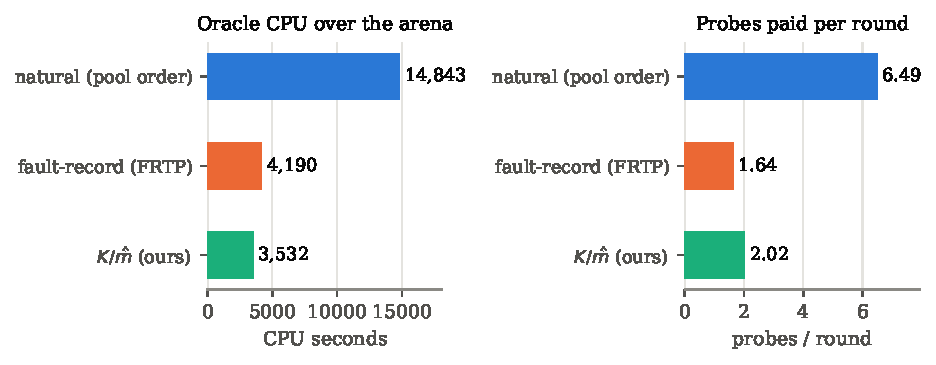
\includegraphics[width=\textwidth]{figures/fig-measured.pdf}
\caption{Measured oracle cost and probe count on the arena. The two panels
rank the policies in \emph{opposite} orders.}
\label{fig:measured}
\end{figure}

\paragraph{Reading.} Against the incumbent the result is large and
uncontroversial: \km\ removes $76.2\,\%$ of the oracle's CPU and is cheaper on
$63$ of $68$ tasks. The interesting comparison is against \frtp, and it is
interesting because the two units of account \textbf{disagree in sign}. \km\
pays $23.3\,\%$ \emph{more} probes and $15.7\,\%$ \emph{less} CPU. The
right-hand column of Table~\ref{tab:measured} shows the mechanism directly:
\frtp\ pays 0.3754\,s per probe --- \emph{more} than the incumbent's
0.3362\,s, because ranking on the kill count steers it towards
exactly the expensive cases that Table~\ref{tab:arena}'s last row predicts ---
while \km\ pays 0.2567\,s, $32\,\%$ less per probe. \km\ does not
find refutations in fewer steps; it finds them in cheaper steps.

This is the pilot's methodological contribution, and it is a caution rather
than a boast. \citet{lou2024aprregression} report executions rather than
seconds for a defensible reproducibility reason, and on a uniform-cost pool
that reporting choice is free. On this pool it would have inverted the
conclusion: measured in executions, \frtp\ wins by $23\,\%$.

\begin{figure}[H]
\centering
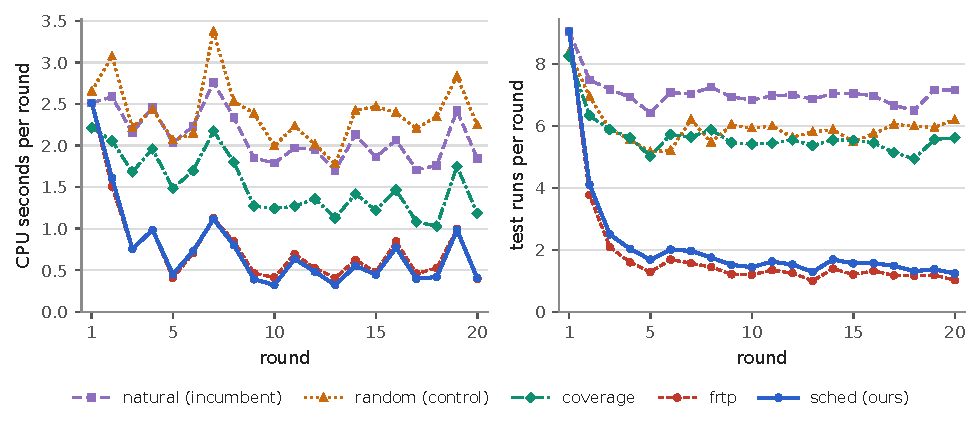
\includegraphics[width=0.72\textwidth]{figures/fig-round-curve.pdf}
\caption{Measured oracle CPU per round. The incumbent never learns; both
memories collapse within about three rounds; \km\ continues to separate from
\frtp\ as its cost model fills in.}
\label{fig:curve}
\end{figure}

Figure~\ref{fig:curve} shows that the ledger is doing what it is supposed to.
In round~1 every policy is identical by construction --- the ledger is empty,
so there is nothing to rank by --- and all three pay about 2\,s. By
round~5 both memory policies have collapsed to roughly a quarter of that. The
two then separate slowly: \frtp\ plateaus around 0.50\,s while \km\
continues down to 0.359\,s by round~20, because its cost estimates
keep improving while \frtp\ has nothing left to learn.

\begin{figure}[H]
\centering
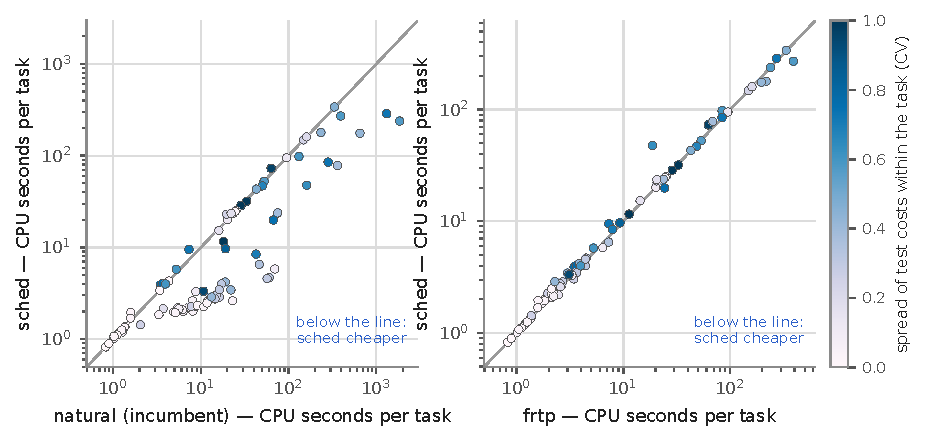
\includegraphics[width=0.52\textwidth]{figures/fig-per-task.pdf}
\caption{Per-task measured CPU, \km\ against \frtp. The win is broad rather
than driven by outliers, but it is not universal.}
\label{fig:pertask}
\end{figure}

Figure~\ref{fig:pertask} is the honest view of the \frtp\ comparison. \km\ is
cheaper on $42$ of $68$ tasks --- a clear majority, not a sweep --- and the
aggregate margin comes partly from the expensive tasks on the upper right,
where the cost spread inside the pool is largest. On cheap, homogeneous pools
the two policies are interchangeable, which is what the theory predicts.

\subsection{Replay Head-to-Head}
\label{sec:pilot-replay}

The replay study puts eight further policies on the same arena without paying
to execute them, by reconstructing from the complete verdict matrix exactly
what each would have probed. It uses $20$ seeds per task. Because the replay
reuses the measured per-case costs, it is a counterfactual over
\emph{orderings}, not a model of execution.

\begin{table}[H]
\centering
\caption{Replay over the arena, $20$ seeds. $\Delta$ is against plain \km;
CIs are a cluster bootstrap over the 68 tasks.}
\label{tab:replay}
\small
\begin{tabular}{@{}l r r r l c@{}}
\toprule
Policy & CPU (s) & probes/rd & $\Delta$ vs \km & 95\,\% CI & sig.\\
\midrule
\code{natural} (pool order)         & 18{,}297.1 & 6.375 & $+589.4\,\%$ & $[+216.8, +990.7]$ & $\star$\\
\code{random} (control)             & 13{,}275.8 & 4.252 & $+400.2\,\%$ & $[+232.6, +549.1]$ & $\star$\\
\code{coverage} ($\mathrm{RTP_{add}}$) & 16{,}611.3 & 5.368 & $+525.8\,\%$ & $[+192.1, +877.0]$ & $\star$\\
\code{cost-only} ($1/\hat m$)       & \phantom{0}8{,}810.6 & 5.083 & $+231.9\,\%$ & $[\phantom{0}+78.9, +403.1]$ & $\star$\\
\code{kill-only} ($K$)              & \phantom{0}2{,}800.9 & 1.305 & $\phantom{00}+5.5\,\%$ & $[\phantom{00}-7.3, \phantom{0}+23.6]$ & \\
\code{km} (\km)                     & \phantom{0}2{,}654.2 & 1.943 & \phantom{00}$0.0\,\%$ & --- & \\
\textbf{\kmc{0.5} (proposed)}       & \phantom{0}\textbf{2{,}409.4} & 1.474 & $\phantom{00}\bm{-9.2\,\%}$ & $[\phantom{0}-15.0, \phantom{00}-1.6]$ & $\bm\star$\\
$K^{0.5}g^{0.25}/\hat m^{0.25}$     & \phantom{0}2{,}366.4 & 1.500 & $\phantom{0}-10.8\,\%$ & $[\phantom{0}-16.1, \phantom{00}-4.2]$ & $\star$\\
\bottomrule
\end{tabular}
\end{table}

Three readings follow.

\emph{The memory term carries most of the effect.} Going from \code{natural} to
\code{kill-only} takes CPU from $18{,}297$ to $2{,}801$. That is the step that
matters most, and it is the step \frtp\ already takes --- which is why \frtp\
is the right baseline and \code{natural} is not.

\emph{Cost alone is not enough.} \code{cost-only} ranks by $1/\hat m$ with no
kill information and lands at $8{,}811$: better than pool order, far worse than
any policy that knows which cases refute. The two terms are not substitutes.

\emph{Additional-greedy coverage does not transfer.} The $\mathrm{RTP_{add}}$
arm reaches $16{,}611$, barely better than pool order and much worse than the
random control. Coverage of the \emph{reference} program is nearly constant
across a contest task's pool --- the median within-task coefficient of
variation of covered-line count is $0.073$ --- so there is almost no marginal
coverage to be greedy about. This is a negative result worth stating plainly:
the strongest classical prioritiser is useless in this setting.

\subsection{How Much to Divide by Cost}
\label{sec:pilot-sweep}

Equation~\eqref{eq:score} leaves the exponent $c$ free, and the two endpoints
are the two published positions: $c = 0$ is the \frtp\ family's kill-only
ranking and $c = 1$ is full cost-cognizance. The sweep measures it.

\begin{figure}[H]
\centering
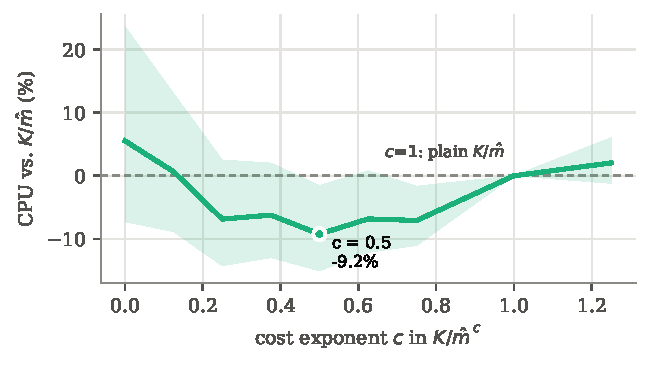
\includegraphics[width=0.72\textwidth]{figures/fig-c-sweep.pdf}
\caption{Cost-exponent sweep, $20$ seeds, paired per task. The optimum is
interior: dividing by cost helps, dividing by the \emph{full} cost
over-corrects.}
\label{fig:csweep}
\end{figure}

The curve is U-shaped with a minimum at $c = 0.5$, which beats plain \km\ by
$9.2\,\%$ (CI $[-15.0, -1.6]$). Both endpoints are worse: $c=0$ costs
$+5.5\,\%$ and $c=1.25$ costs $+2.0\,\%$, neither significantly different from
\km. The interpretation is that $\hat m$ is a noisy online estimate, and a
square root is the standard way to use a noisy denominator without letting one
cheap-looking early measurement dominate the ranking. The practical conclusion
for Phase~2 is that $c$ must be a tuned parameter with a declared default, not
a constant fixed at $1$ by the name of the method.

A companion sweep added the marginal-coverage term $g$ of
Equation~\eqref{eq:additional} as a third factor at fifteen $(a,b,c)$
combinations. Of the fifteen, twelve have confidence intervals straddling
zero; the largest effect at the operating point $a{=}1, c{=}0.5$ is
$-2.2\,\%$ with CI $[-5.0, +0.9]$. Coverage is therefore \textbf{dropped from
the proposed score}: it costs a tracing pass per case and buys nothing
measurable.

\subsection{Soundness Check}
\label{sec:soundness}

Definition~\ref{def:soundness} says no ordering can change which patches are
accepted. The measured runs confirm it: all three policies accepted exactly
$6$ patches over the $6{,}800$ rounds each. A discrepancy here would have been
a soundness bug rather than a finding, and the check is cheap enough to repeat
on every cell in Phase~2.

\subsection{Reproducibility}

Every number in this section is regenerated from three input files --- the
verdict matrix, the per-case cost table and the per-case coverage table ---
by the scripts shipped under \code{report/scripts/}. The replay head-to-head
and the exponent sweep were re-run from scratch for this document and
reproduce the stored values to the printed precision; the measured block is a
direct aggregation of the $33{,}000$-row round log. Generated artefacts are
under \code{report/data/}.

\section{Discussion}
\label{sec:pilot-discussion}

\paragraph{What the evidence supports.} Three claims are supported at the
pilot's scale. The oracle's cost in a counterexample-guided repair loop is
dominated by probe ordering, and a per-case memory removes about three quarters
of it. A cost-aware ranking beats the published kill-count ranking by a
further $15.7\,\%$ of CPU, with the margin coming from cheaper probes rather
than fewer ones. And the unit of account is not neutral on this corpus: CPU and
executions order the policies oppositely, so a prioritisation result reported
in executions alone does not transfer to a deployment that pays seconds.

\paragraph{What it does not support.} The pilot says nothing about the
proposer. RQ3 and RQ4 --- whether a counterexample keyed to a test case and
phrased as a positive requirement renormalises the patch distribution, and at
what disclosure that turns into fitting the shown tests --- are untouched,
because the \cegmem\ data was collected under a prohibition-style prompt and no
replay can manufacture a counterfactual model call. It also says nothing about
scale: $68$ tasks is a pilot, the arena is restricted to tasks whose cost and
coverage passes finished, and that restriction is not random with respect to
task cost. Finally, the $15.7\,\%$ margin over \frtp\ has a wide interval
($[-28.9, -5.1]$) and holds on $42$ of $68$ tasks; it is a real effect at this
scale, not a settled magnitude.

\paragraph{Threats carried into Phase 2.} Three are worth naming now. The
arena's selection is cost-correlated, so the full corpus may show a smaller
margin. The replay reuses one cost measurement per case rather than sampling
the cost distribution, which understates variance --- the measured block exists
precisely so the headline does not depend on the replay. And \code{gpt-4o-mini}
produced every patch in the matrix, so the patch population, and therefore the
kill structure the ledger learns, is one model's.

\chapter{Evaluation Plan}
\label{ch:evaluation}

Nothing in this chapter is a result. Every figure below is a target or a
protocol; the only measured evidence in this document is
Section~\ref{sec:pilot}.

\section{Metrics}
\label{sec:metrics}

The study does not collapse into a single figure of merit, because the two
halves of the loop spend different resources and a composite would let one pay
for the other. Metrics are grouped by the resource they account for.

\begin{table}[H]
\centering
\caption{Oracle-side metrics (RQ1, RQ2).}
\label{tab:metrics-oracle}
\small
\begin{tabularx}{\textwidth}{@{}>{\raggedright\arraybackslash}p{0.19\textwidth} X X@{}}
\toprule
Metric & Definition & Success criterion\\
\midrule
CPU seconds / episode & \code{getrusage} delta summed over paid probes; paired per cell under common random numbers & \km\ below \code{natural}, \code{fault-record} and \code{coverage}, beyond the cluster bootstrap's interval\\
\code{test\_calls} / episode & Probe count, reported alongside CPU because the prioritisation literature reports executions & Reported for every arm; \emph{not} a success criterion on its own\\
CPU per probe & CPU $\div$ probes; isolates ``cheaper'' from ``fewer'' & Diagnostic; the pilot's mechanism claim lives here\\
Stepwise decomposition & Paired $\Delta$ CPU for each one-variable step of the ablation ladder & At least one step clears the interval\\
\bottomrule
\end{tabularx}
\end{table}

\begin{table}[H]
\centering
\caption{Proposer-side metrics (RQ3, RQ4).}
\label{tab:metrics-proposer}
\small
\begin{tabularx}{\textwidth}{@{}>{\raggedright\arraybackslash}p{0.19\textwidth} X X@{}}
\toprule
Metric & Definition & Success criterion\\
\midrule
\code{duplicate\_rate} & $1 - \text{distinct}/\text{total}$ patches in an episode. RQ3's primary & Falls against \code{no-mem} (independent repeated sampling)\\
\code{success@B} & Share of cells repaired within budget $B$ & Rises, or at minimum does not fall, where \code{duplicate\_rate} falls\\
\code{first\_accept\_round} & Round of first acceptance & Reported paired\\
Prompt / completion tokens, USD & The proposer's bill, since the repair literature prices in tokens~\citep{hidvegi2024cigar} & Reported for every Block-B arm\\
Disclosure leakage & Of refuted patches, the share whose refuting set is \emph{disjoint} from what the prompt showed & Falls monotonically as disclosure rises, or RQ4's axis does not exist\\
\bottomrule
\end{tabularx}
\end{table}

\paragraph{Guaranteed, not measured.} \code{success@B} and
\code{first\_accept\_round} are identical across every replay arm on every
cell, by Definition~\ref{def:soundness}. RQ1 is a pure cost claim; a gap there
is a soundness bug, and the grid asserts it rather than reporting it.

\section{The Arm Roster}
\label{sec:arms}

Twenty-two arms, in two blocks that differ in what they cost to run.

\paragraph{Block A --- replay arms, zero model calls (13).} Every arm here
differs only in the probe order, so the patches are drawn once and reused,
and a new arm costs nothing but CPU: \code{full-suite}, \code{no-mem},
\code{natural}, \code{random}, \code{fault-record}, \code{cost-only},
\code{kill-only}, \code{coverage}, \code{km}, \code{km-cs-median},
\code{km-cs-q75}, \code{km-bucket}, \code{km-explore0}.

\paragraph{Block B --- steered arms, one model-call grid each (9).} For these
the round-$t$ prompt is a function of the ledger at round $t$, so the draw and
the schedule are not separable: \code{km+steer}, \code{km+steer-pass},
\code{km+exclusion}, \code{km+chat}, \code{km+steer-k1}, \code{km+steer-k3},
\code{km+steer-sample}, \code{km+steer-noreq}, \code{km+steer+vs}.

Two framing points govern how the roster is read, and both are consequences of
Chapter~\ref{ch:related}.

\begin{itemize}[leftmargin=*]
\item \textbf{\code{natural} is the incumbent, not a neutral control.} Sorting
by filename is not a scheduling decision anyone made; it is what any
implementation gets for free. It is also not arbitrary --- AtCoder's naming
puts the small, public, highly discriminating cases first --- so it is
\emph{better} than chance, which is exactly why the pilot's random control is
cheaper than it. \code{random} is the control.
\item \textbf{\code{no-mem} is the RQ3 baseline, and it is a strong one.} It
redraws independently every round under a policy-free nonce, which is precisely
independent repeated prompting --- the strategy
\citet{chen2025conversational} measured at $23$ bugs repaired against
conversational repair's $18$. Block B must beat \code{no-mem}; beating
\code{natural} proves nothing on the proposer side.
\end{itemize}

\section{Ablation Ladder}
\label{sec:ablation}

An ablation chain must change one thing per step or it cannot attribute.
\code{fault-record} $\to$ \code{km} changes two --- a count becomes a rate,
\emph{and} the rate is divided by cost --- so the ladder is built to separate
them.

\begin{table}[H]
\centering
\caption{The ablation ladder. One variable per step.}
\label{tab:ablation}
\small
\begin{tabularx}{\textwidth}{@{}l l X@{}}
\toprule
Step & What changes & What it would mean if it does not clear the interval\\
\midrule
\code{natural} $\to$ \code{cost-only}      & cost enters, no kill info & Cost alone is not a usable signal (pilot: it is not, on its own)\\
\code{natural} $\to$ \code{kill-only}      & kill rate enters, no cost & The memory term is ornament\\
\code{natural} $\to$ \code{fault-record}   & the published baseline's step & \frtp\ does not reproduce\\
\code{fault-record} $\to$ \code{kill-only} & a \textbf{count} becomes a \textbf{rate} & Reading the denominator buys nothing\\
\code{kill-only} $\to$ \code{km}           & the rate is divided by cost & Cost-awareness is ornament\\
\code{km} $\to$ \kmc{c}                    & the exponent is tuned & $c$ need not be a parameter (pilot: it does)\\
\bottomrule
\end{tabularx}
\end{table}

\section{Sensitivity}

Four arms ask whether RQ1's answer survives the project's own design choices,
and one asks the same of RQ3. They belong in threats to validity, not in the
question count: \code{km-cs-median} and \code{km-cs-q75} vary the cold-start
rule for $\hat m$; \code{km-bucket} replaces the continuous score with buckets;
\code{km-explore0} removes exploration --- and is additionally a
\emph{precondition} of RQ4, because without exploration a task whose first
probe refutes everything reaches the prompt with one fact, $k{=}2$ degenerates
to $k{=}1$, and the $k$ sweep compares $k{=}1$ against itself;
\code{km+steer+vs} diversifies the \emph{draw} rather than the evidence.

\section{Protocol and Tooling}

\begin{table}[H]
\centering
\caption{Tools and their role.}
\label{tab:tools}
\small
\begin{tabularx}{\textwidth}{@{}l X@{}}
\toprule
Tool & Role\\
\midrule
ConDefects~\citep{wu2024condefects} & Fault corpus, test pools and reference outputs\\
Python \code{subprocess} + \code{resource} & The sandbox: one program, one input, hard timeout, CPU via \code{getrusage}\\
OpenAI-compatible endpoint & The proposer; one model per grid, with a cross-run response cache\\
\code{caster} CLI (ten verbs) & Corpus freeze, phase-1 draw, phase-2 grid walk, full-scan audit, shard merge, analysis, HTML report\\
Cluster bootstrap + Wilcoxon & Interval estimation over tasks; paired tests over per-task totals\\
\bottomrule
\end{tabularx}
\end{table}

\paragraph{Grid.} The corpus gate admits every sound fault rather than a
screened subset, producing on the order of $1{,}244$ faults; banding by pool
size and contest era happens in analysis, after treatment. Cells are
$(\text{task} \times \text{seed} \times \text{policy})$, written atomically and
resumably, with the done-index written after the rows. A merge runs six audits
before anything is treated as evidence.

\paragraph{Common random numbers.} Round~1 carries no facts, so a steered
prompt must be byte-identical to an unsteered one and share its cache entry.
That works only if the draw nonce is \code{task|seed|round} and is
\emph{not} a function of the policy. Deriving it from the cell key --- which
does contain the policy --- would kill CRN silently while buying every
completion once per arm.

\section{Baseline Comparisons}

\begin{table}[H]
\centering
\caption{Tier A --- reproduced head-to-head on our corpus.}
\label{tab:tiera}
\small
\begin{tabularx}{\textwidth}{@{}l X l@{}}
\toprule
System & Role & Expected outcome\\
\midrule
\code{natural} & The incumbent order & \km\ substantially cheaper (pilot: $-76\,\%$)\\
\frtp~\citep{qi2013frtp} & The published repair-loop prioritiser, ranking on the kill count & \km\ cheaper in CPU, \emph{more expensive} in executions (pilot: $-15.7\,\%$ / $+23.3\,\%$)\\
$\mathrm{RTP_{add}}$~\citep{rothermel2001prioritizing} & The strongest classical prioritiser & No better than pool order here (pilot: confirmed)\\
\code{no-mem} & Independent repeated sampling~\citep{chen2025conversational} & The RQ3 baseline Block B must beat\\
\code{km+chat} & A \textsc{ChatRepair}-style transcript~\citep{xia2024chatrepair} & Higher duplicate rate and faster prompt growth than the requirement contract\\
\bottomrule
\end{tabularx}
\end{table}

\begin{table}[H]
\centering
\caption{Tier B --- cited qualitatively from the original papers; not
reproducible within this project's budget.}
\label{tab:tierb}
\small
\begin{tabularx}{\textwidth}{@{}l X X@{}}
\toprule
System & Reported result & Relation to this work\\
\midrule
APR\,$\times$\,RTS~\citep{lou2024aprregression} & 2.53M patches; selection beats prioritisation in Java & Different setting: no call graph to select on; and they report executions, we report CPU\\
\textsc{CigaR}~\citep{hidvegi2024cigar} & 127K vs 467K tokens / bug & Complementary currency: they cut the proposer's bill, we cut the oracle's\\
\textsc{ChatRepair}~\citep{xia2024chatrepair} & 162/337 bugs at \$0.42 each & The conversational incumbent our Block-B contract is measured against\\
MPP~\citep{venugopal2020mpp} & Modification-point-aware patch killing count & Same missing denominator and missing cost as \frtp\\
\bottomrule
\end{tabularx}
\end{table}

\section{Threats to Validity}

\paragraph{Construct.} Cost is CPU, not wall clock or money. A deployment that
pays for wall clock on a loaded machine, or for a managed test service priced
per invocation, would weight the two units differently --- and the pilot shows
those weightings disagree. Both are therefore reported for every arm.

\paragraph{Internal.} The ledger learns from the patches the proposer happens
to produce, so policy and data are coupled within an episode. Common random
numbers hold round~1 identical across arms, and the full-scan \code{audit} pass
establishes the kill matrix independently of any arm, so no arm's ordering can
contaminate the cost table.

\paragraph{External.} One benchmark, one language, one proposer model, and a
competitive-programming fault distribution with small single-file programs and
whole-program probes. Transfer to Java projects with method-level suites is not
claimed; the setting there is the one where
\citet{lou2024aprregression} find selection to dominate.

\paragraph{Conclusion.} Per-task totals are not independent across seeds, so
intervals come from a cluster bootstrap over tasks rather than over cells, and
paired tests run on per-task totals.

\chapter{Summary and Future Plan}
\label{ch:summary}

\section{Summary}

A counterexample-guided repair loop spends a counterexample twice and, in the
usual implementation, wastes it both times: once by running the oracle in an
order nobody chose, and once by letting the proposer redraw from the mode it
has just drawn from. This proposal addresses the first waste and designs for
the second.

The route to it ran through a previous study. \cegmem\ gave the repair loop a
memory keyed by a failure type --- edit location crossed with violated property
--- and that memory worked: oracle calls per episode fell from $11.11$ to
$1.57$, and the repair rate rose from $0.526$ to $0.581$ over $309$ tasks.
Reading its columns carefully is what produced the present question. Oracle
\emph{calls} fell $7.07\times$, but sandbox \emph{runs} fell only $2.35\times$,
because a class-keyed index decides \emph{whether} to pay the oracle and has
nothing to say about \emph{how} the oracle spends once it is paid. A failure
class is a category; a test case is an observation; only the latter can be
ordered, costed, or phrased to a model as a requirement.

\caster\ therefore re-keys the memory by test case and ranks probes by
$K/\hat m^{\,c}$ --- an online Beta-posterior kill rate over an online mean CPU
cost. The preliminary study of Section~\ref{sec:pilot}, run on the frozen
\cegmem\ data because only that data carries the complete patch~$\times$~case
verdict matrix an exact counterfactual replay needs, establishes the following
on $68$ tasks, $2{,}523$ cases and $4{,}670$ patches:

\begin{itemize}[leftmargin=*,itemsep=3pt]
\item \textbf{Against the incumbent}, measured over $6{,}800$ rounds per
policy, \km\ removes $76.2\,\%$ of oracle CPU (95\,\% CI $[-84.9, -61.2]$,
$p = 1.7\times10^{-11}$), and is cheaper on $63$ of $68$ tasks.
\item \textbf{Against the published \frtp\ baseline}, \km\ removes a further
$15.7\,\%$ of CPU (CI $[-28.9, -5.1]$, $p = 0.011$, $42$ of $68$ tasks)
\emph{while paying $23.3\,\%$ more probes}. The mechanism is visible in the
cost per probe: \frtp\ pays 0.375\,s, which is \emph{more} than the
incumbent's 0.336\,s, because ranking on kill count steers it
towards expensive cases; \km\ pays 0.257\,s.
\item \textbf{The unit of account is not neutral.} CPU and executions rank the
two policies oppositely on this corpus, so a prioritisation result reported in
executions --- as the literature reports it, for good reproducibility
reasons --- would have inverted the conclusion.
\item \textbf{The exponent is a parameter, not a constant.} The cost-exponent
sweep has an interior optimum at $c = 0.5$, beating plain \km\ by $9.2\,\%$
(CI $[-15.0,-1.6]$); both $c{=}0$ and $c{=}1.25$ are worse.
\item \textbf{A negative result.} Additional-greedy coverage, the strongest
classical prioritiser, performs barely better than pool order and worse than
random here, because reference coverage is nearly constant across a contest
task's pool (median within-task CV $0.073$). It is dropped from the score.
\item \textbf{Soundness holds.} All three measured policies accepted exactly
the same number of patches, as Definition~\ref{def:soundness} requires.
\end{itemize}

What the pilot does not establish is equally important. It says nothing about
the proposer: RQ3 and RQ4 are untouched, because no replay can manufacture a
counterfactual model call. It is a pilot at $68$ tasks, drawn from a subset
whose selection correlates with cost. And every patch in the matrix came from
one model.

\section{Future Direction}
\label{sec:future}

The remaining work is organised so that the pipeline is frozen before the
evaluation runs, rather than tuned while it runs. \textbf{Every item below is
Phase~2 work and none of it has been executed.}

\begin{itemize}[leftmargin=*,itemsep=4pt]
\item \textbf{Run the Block-A grid on the full corpus.} Thirteen replay arms
over roughly $1{,}244$ gated faults, with the \code{audit} full-scan pass
establishing the kill matrix and the cost table independently of any arm.
This re-establishes RQ1 at scale and runs the ablation ladder of
Section~\ref{sec:ablation} for RQ2.
\item \textbf{Fix $c$ by protocol, not by hindsight.} The pilot's $c = 0.5$
was selected on the pilot arena. Phase~2 declares $c$ before the corpus run and
reports the sweep as sensitivity, so the headline is not a selected maximum.
\item \textbf{Implement and run Block B.} Nine steered arms, each a full
model-call grid. This is the first test of the proposal's second half --- that
a counterexample keyed to a test case and phrased as a positive requirement
moves the proposal distribution where a prohibition and a transcript do not ---
measured against independent repeated sampling, which is the published stronger
strategy~\citep{chen2025conversational}.
\item \textbf{Measure the disclosure dose (RQ4).} The $k$ sweep and the
disclosure sweep are one dose-response curve; \code{km-explore0} must be in
place first or the curve compares $k{=}1$ against itself.
\item \textbf{Report both bills together.} The oracle's CPU and the proposer's
tokens are halves of one cost. \textsc{CigaR} optimised the second and reported
$127$K against $467$K tokens per bug~\citep{hidvegi2024cigar}; this project
optimises the first and should report the pair rather than either alone.
\item \textbf{Beyond this setting (thesis horizon).} Whole-program probes and
single-file faults are what make selection unavailable and prioritisation the
only lever. Carrying the cost-aware ledger into a setting with method-level
suites, where selection \emph{is} available~\citep{lou2024aprregression}, is
the natural generalisation and is out of scope here.
\end{itemize}

\section{Limitations}

\begin{table}[H]
\centering
\caption{Limitations and planned mitigations.}
\label{tab:limitations}
\small
\begin{tabularx}{\textwidth}{@{}X X X@{}}
\toprule
Limitation & Impact & Mitigation\\
\midrule
The \caster\ grid has not been run; evidence is a pilot on the predecessor's data & RQ1 is established at $68$ tasks, not at corpus scale; RQ2 only partially & Phase~2 Block-A grid on $\approx 1{,}244$ faults with the full ablation ladder\\
Arena selection correlates with cost (only tasks whose cost and coverage passes finished) & The $15.7\,\%$ margin over \frtp\ may shrink & The full corpus admits every sound fault; no pre-treatment screen\\
One proposer model (\code{gpt-4o-mini}) produced every patch in the matrix & The kill structure the ledger learns is one model's & A second proposer in Phase~2 sensitivity\\
The replay reuses one cost sample per case & Understates cost variance & The headline rests on the re-executed block, not the replay\\
$c = 0.5$ was selected on the same arena it is reported on & A selected maximum is optimistically biased & Declare $c$ before the corpus run; report the sweep as sensitivity\\
Whole-program, single-file, stdout-compared faults & No claim transfers to project-scale Java repair & Stated as external threat; selection-capable settings are future work\\
CPU is the cost; money and wall clock are not & A differently priced deployment weights the units differently & Both CPU and executions reported for every arm\\
\bottomrule
\end{tabularx}
\end{table}

\section{Timeline}

The project runs across the 2026 calendar year in two phases separated by the
institutional summer break. Phase~1 covers the work reported here: the
\cegmem\ study that generated the question, the literature consolidation, the
\caster\ implementation and its unit tests, and the pilot. Phase~2 covers the
grid, the steered block, and the writing.

\begin{figure}[H]
\centering
\resizebox{\textwidth}{!}{%
\begin{ganttchart}[
  hgrid, vgrid,
  x unit=0.62cm, y unit title=0.58cm, y unit chart=0.52cm,
  title/.style={fill=none,draw=black!55},
  title label font=\scriptsize\bfseries,
  bar/.style={fill=bkblue!50,draw=bkblue,rounded corners=1pt},
  bar height=0.52,
  group/.style={fill=bkblue!85,draw=none},
  group right shift=0, group left shift=0,
  bar label font=\scriptsize,
  group label font=\scriptsize\bfseries,
  milestone label font=\scriptsize\itshape
]{1}{17}
\gantttitle{2026}{12} \gantttitle{2027}{5} \\
\gantttitlelist{"J","F","M","A","M","J","J","A","S","O","N","D","J","F","M","A","M"}{1} \\
\ganttgroup{Phase 1 -- premise and proposal}{1}{11} \\
\ganttbar{\cegmem\ study (typed memory)}{1}{6} \\
\ganttbar{Literature consolidation}{7}{8} \\
\ganttbar{\caster\ design and implementation}{9}{10} \\
\ganttbar{Unit tests and invariants}{9}{10} \\
\ganttbar{Cost / coverage measurement passes}{10}{11} \\
\ganttbar{Pilot: replay + re-execution}{11}{11} \\
\ganttbar{Proposal writing}{11}{11} \\
\ganttmilestone{Proposal defence}{11} \\
\ganttgroup{Phase 2 -- the grid}{12}{17} \\
\ganttbar{Corpus freeze; \code{audit} full scan}{12}{13} \\
\ganttbar{Block-A grid (13 arms)}{13}{14} \\
\ganttbar{Block-B implementation and grid (9 arms)}{14}{15} \\
\ganttbar{Disclosure sweep (RQ4)}{15}{16} \\
\ganttbar{Sensitivity, threats, writing}{16}{17} \\
\ganttmilestone{Final defence}{17}
\end{ganttchart}}
\caption{Project timeline. Everything up to and including the proposal-defence
milestone has been carried out; every bar below it is planned work.
Deliverables per work package are in Table~\ref{tab:workpackages}.}
\label{fig:timeline}
\end{figure}

\begin{table}[H]
\centering
\caption{Work packages by phase.}
\label{tab:workpackages}
\small
\begin{tabularx}{\textwidth}{@{}l l X X@{}}
\toprule
Phase & Period & Main focus & Deliverable\\
\midrule
\multirow{5}{*}{Phase 1} & Jan--Jun & \cegmem: typed memory, the $309$-task grid & The premise, and the residual that generated RQ1\\
 & Jul--Aug & Literature consolidation & Related-work matrix; the gap statement of Sec.~\ref{sec:gap}\\
 & Sep--Oct & \caster\ design and implementation & Ten verbs; the three module boundaries; 263 unit tests\\
 & Oct--Nov & Cost and coverage measurement passes & \code{cost\_all}, \code{cov\_all}, the verdict matrix\\
 & Nov & Pilot and proposal & Sec.~\ref{sec:pilot}; this document; defence\\
\midrule
\multirow{5}{*}{Phase 2} & Dec--Jan & Corpus freeze; \code{audit} full scan & Kill matrix and frozen cost table, arm-independent\\
 & Jan--Feb & Block-A grid, 13 arms & RQ1 at corpus scale; the RQ2 ablation ladder\\
 & Feb--Mar & Block-B implementation and grid, 9 arms & RQ3: duplicate rate against repeated sampling\\
 & Mar--Apr & Disclosure sweep & RQ4 dose-response curve\\
 & Apr--May & Sensitivity, threats, writing & Final manuscript and defence\\
\bottomrule
\end{tabularx}
\end{table}

Two buffers are built into the plan. The evaluation protocol --- the corpus
gate, the pool order, the cost table and the declared value of $c$ --- is
frozen at the end of Phase~1, so unexpected behaviour in Phase~2 can be
analysed rather than hidden by continuous retuning. And because Block~A costs
no model calls, the thirteen replay arms can be re-run freely whenever the
analysis changes, which is what makes the ablation ladder affordable at all.


% ======================= BACK MATTER ========================
\cleardoublepage
\phantomsection
\addcontentsline{toc}{chapter}{References}
\renewcommand{\bibname}{References}
\bibliographystyle{unsrtnat}
\bibliography{refs}

\end{document}
